
\section{Changes to Dataset} % Top level section
\begin{fullwidth}We need to change some properties to prepare the dataset before feeding it to a model\dots\end{fullwidth}

\subsection{Updates to resolution}
\begin{fullwidth}As we mentioned earlier, we decreased the resolution of all images in the whole dataset to make it more manageable. \end{fullwidth}
See \ref{fig:rescale_res_result}.

\subsection{File extension formatting}
\begin{fullwidth}
Most images were of \verb|.JPG| format and some of \verb|.JPEG| and \verb|.PNG| format. 
To make all these images the same file format we choose to convert them all to the PNG format. 
We will choose \verb|.PNG| because this file format stores details of the image as extra metadata per image. 
The advantage of this is that the image doesn't lose details when augmenting it. 
The disadvantage is that the size of the image increases.
\end{fullwidth}

\subsection{Applying grayscale}
\sidenote{We need to apply a grayscale effect to remove the BGR-channels currently present in the image. 
The image contains colours which might interfere with classification and makes it harder to bring out the details.
Applying Grayscale makes sure those details are easier to bring out in the next preprocessing techniques.}
\begin{figure}[H] % [H] forces the figure to be output where it is defined in the code (it suppresses floating)
	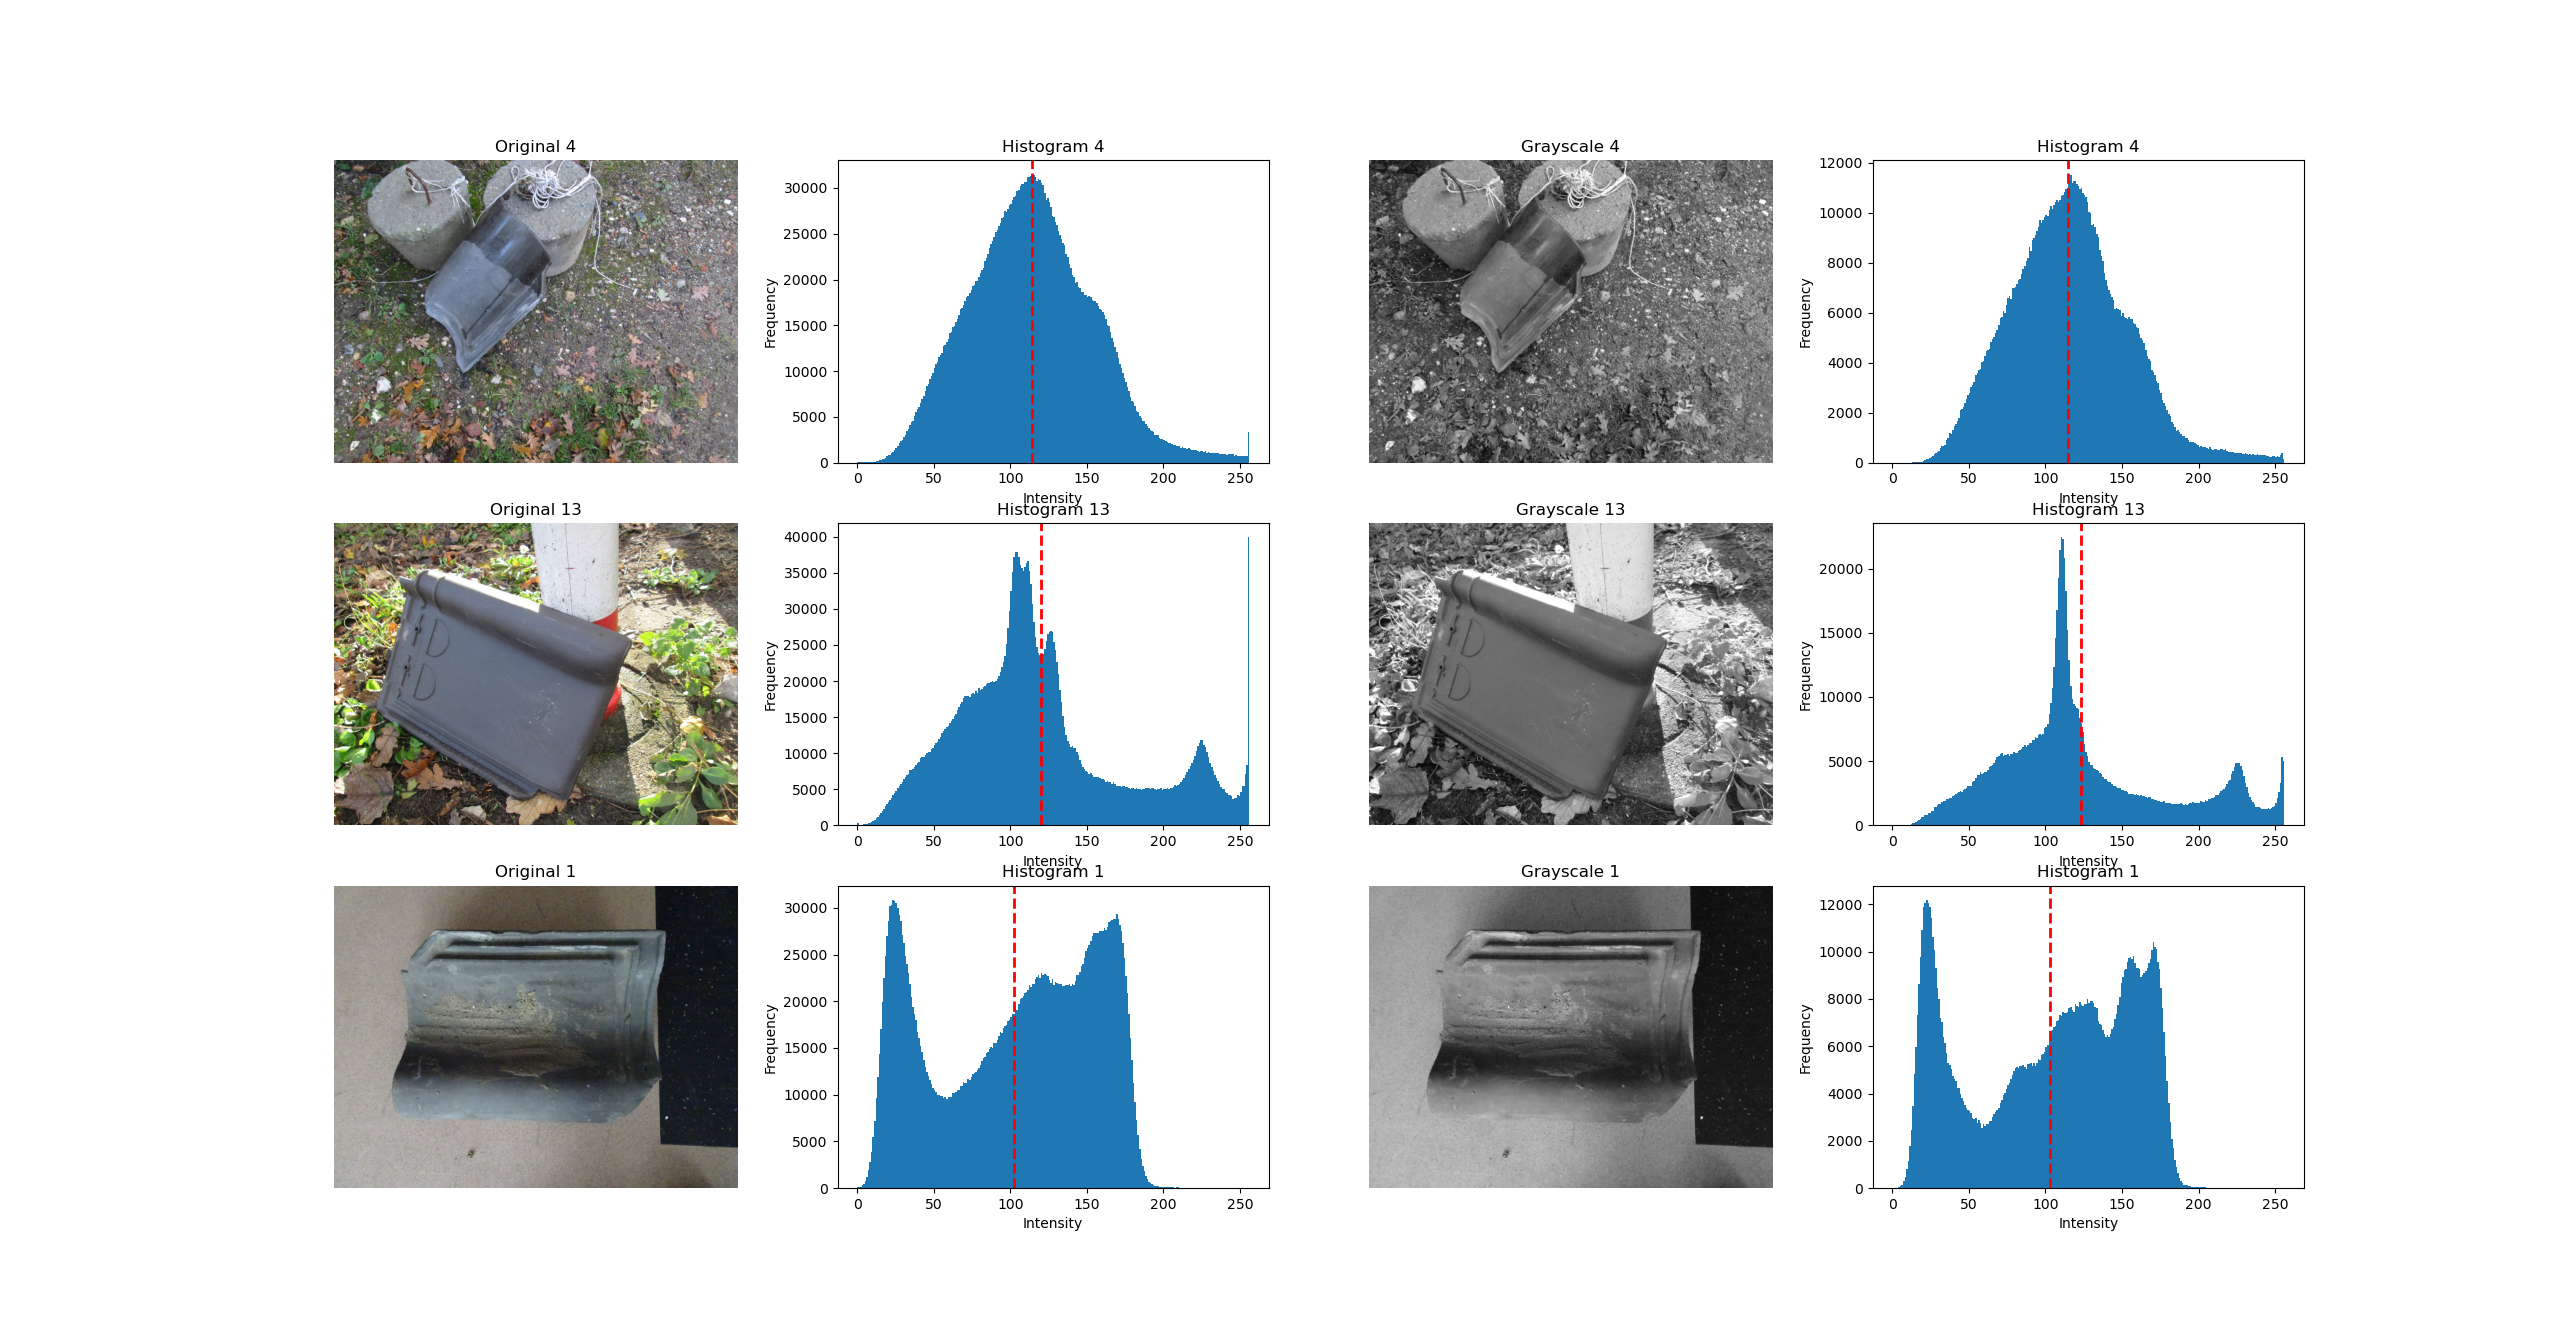
\includegraphics[width=\linewidth]{grayscale_graph_histogram.png}
	\caption{Grayscale of images plot}
	\label{fig:grayscale_graph_histogram} % Label for referencing this figure in the text automatically
\end{figure}

\newpage
\subsection{Applying normalization}
\sidenote[][1cm]{After grayscaling, normalization needs to be applied to normalize contrast. 
Doing this removes some glare or extreme lighting effects caused by the camera lens.}
\begin{figure}[H] % [H] forces the figure to be output where it is defined in the code (it suppresses floating)
	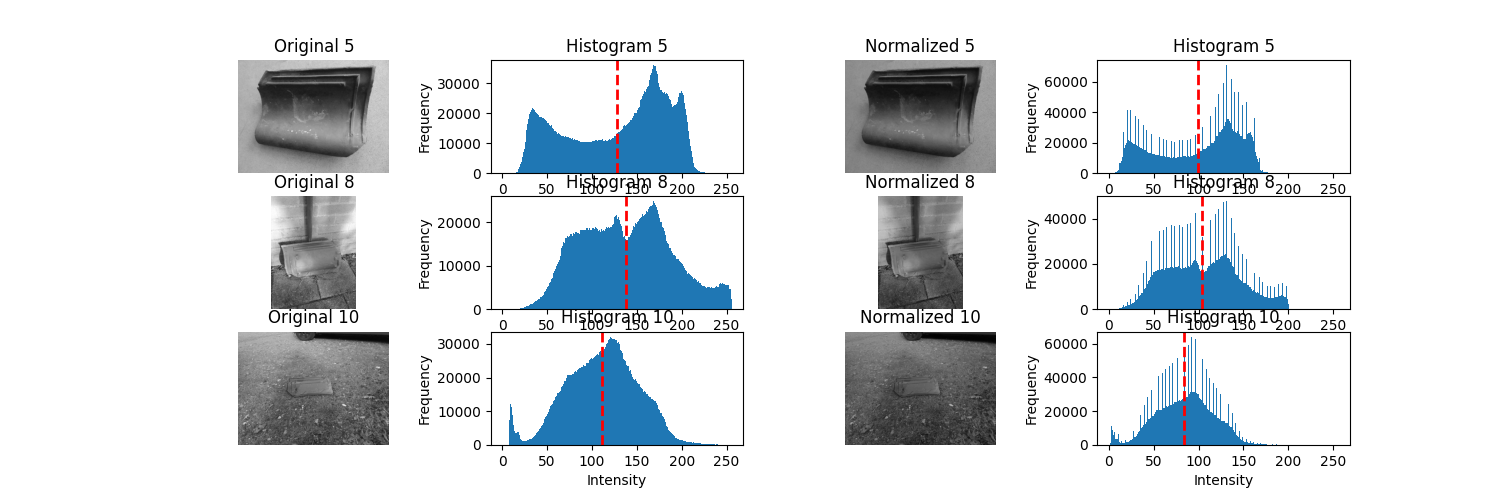
\includegraphics[width=\linewidth]{normalization_conversion_before_after.png}
	\caption{Normalization of images plot}
	\label{fig:normalization_conversion_before_after} % Label for referencing this figure in the text automatically
\end{figure}

% \newpage
\subsection{Applying CLAHE}
\sidenote{Lastly, CLAHE is applied to bring out more details. 
CLAHE does this to dampen some of the higher pixel values and placing them below the average threshold, 
so that details appear more sharp.}
\begin{figure}[H] % [H] forces the figure to be output where it is defined in the code (it suppresses floating)
	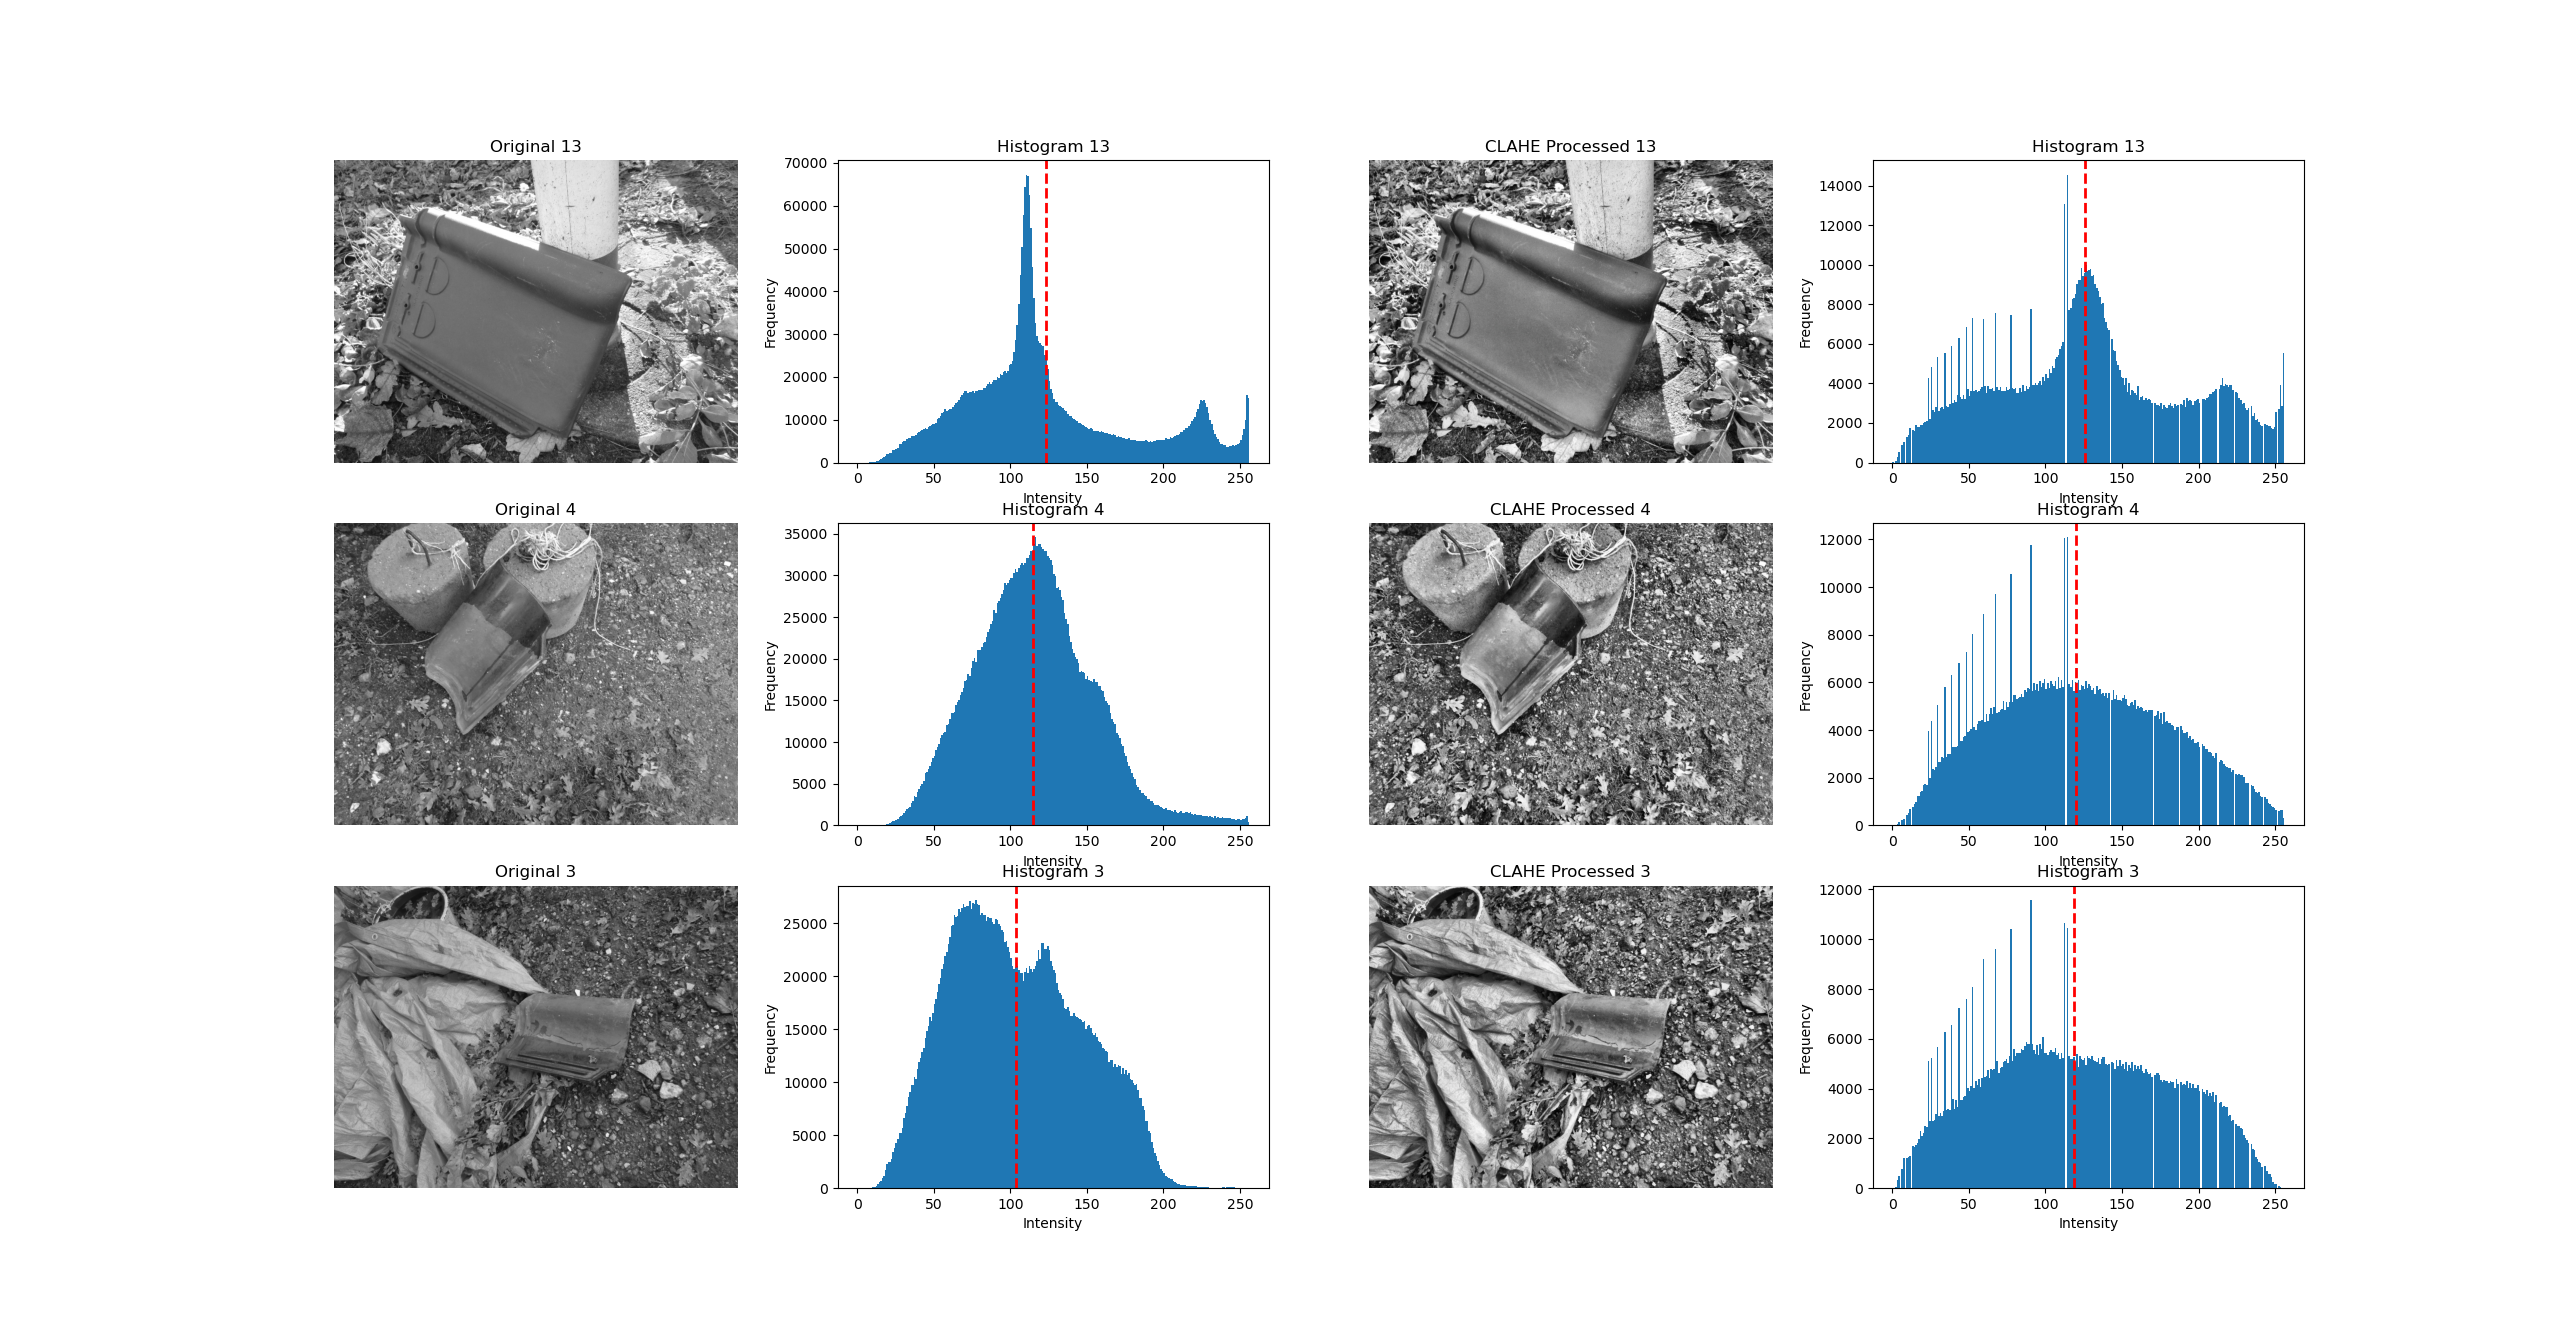
\includegraphics[width=\linewidth]{clahe_graph_histogram.png}
	\caption{CLAHE of images plot}
	\label{fig:clahe_graph_histogram} % Label for referencing this figure in the text automatically
\end{figure}

\newpage
\subsection{Splitting data based on side of rooftile}
The dataset consists of 2 types of images per rooftile:
\begin{itemize}
	\item Picture from the top
	\item Picture from the bottom
\end{itemize}

\sidenote{As described in the first section, all folders are on the same level. This means that top and bottom images are on the same directory level as well. 
We don't want that. What we want is to split the folders based on the top/bottom side of the rooftile so we can train two models, one for each side of the rooftile.
We end up with the following folderstructure (Please note that this does not include all folders):}

\begin{forest}
	for tree={
		font=\ttfamily,
		grow'=0,
		child anchor=west,
		parent anchor=south,
		anchor=west,
		calign=first,
		edge path={
			\noexpand\path [draw, \forestoption{edge}]
			(!u.south west) +(7.5pt,0) |- node[fill,inner sep=1.25pt] {} (.child anchor)\forestoption{edge label};
		},
		before typesetting nodes={
			if n=1
			{insert before={[,phantom]}}
			{}
		},
		fit=band,
		before computing xy={l=15pt},
	}
	[dataset
		[b
			[d0000\_b\_blw\_g\_OVH
				[d0000\_b\_blw\_g\_OVH (1).png]
				[d0000\_b\_blw\_g\_OVH (2).png]
				[d0000\_b\_blw\_g\_OVH (3).png]
			]
			[d0001\_b\_blw\_n\_TDN44
				[d0001\_b\_blw\_n\_TDN44 (1).png]
				[d0001\_b\_blw\_n\_TDN44 (2).png]
				[d0001\_b\_blw\_n\_TDN44 (3).png]
			]
		]
		[o
			[d0000\_o\_blw\_g\_OVH
				[d0000\_o\_blw\_g\_OVH (1).png]
				[d0000\_o\_blw\_g\_OVH (2).png]
				[d0000\_o\_blw\_g\_OVH (3).png]
			]
			[d0001\_o\_blw\_n\_TDN44
				[d0001\_o\_blw\_n\_TDN44 (1).png]
				[d0001\_o\_blw\_n\_TDN44 (2).png]
				[d0001\_o\_blw\_n\_TDN44 (3).png]
			]
		]
	]
\end{forest}


\newpage
\subsection{Training and testing data}

% \begin{fullwidth}
% \end{fullwidth}

\sidenote[][]{After splitting the top and bottom side of the rooftiles we will split the data into training and testing but there is a small catch: 
we want to keep the proportion of the different rooftiles within each set.
To do this we will use stratified splitting.
This is so we don't dont end up with a lot of one type of rooftile and a lot less of another type in either training or testing set.
A training ratio of $70\%$ will be used as default ratio.
We will use "train\_test\_split" from Python's library "sklearn" for splitting into training and testing.
By doing stratified splitting, we end up with the folderstructure you can see on the left side of the page.}

% \sidenote[][]{}

% \sidenote[][]{}

% \sidenote[][]{}

\begin{forest}
    for tree={
        font=\ttfamily\small,
        grow'=0,
        child anchor=west,
        parent anchor=south,
        anchor=west,
        calign=first,
        edge path={
            \noexpand\path [draw, \forestoption{edge}]
            (!u.south west) +(7.5pt,0) |- node[fill,inner sep=1.25pt] {} (.child anchor)\forestoption{edge label};
        },
        before typesetting nodes={
            if n=1
            {insert before={[,phantom]}}
            {}
        },
        fit=band,
        before computing xy={l=15pt},
        s sep=2pt, % Adjust vertical spacing
    }
    [dataset
        [test
            [b
                [d0000\_b\_blw\_g\_OVH
                    [d0000\_b\_blw\_g\_OVH (1).png]
                    [d0000\_b\_blw\_g\_OVH (2).png]
                ]
                [d0001\_b\_blw\_n\_TDN44
                    [d0001\_b\_blw\_n\_TDN44 (1).png]
                    [d0001\_b\_blw\_n\_TDN44 (2).png]
                ]
            ]
            [o
                [d0000\_o\_blw\_g\_OVH
                    [d0000\_o\_blw\_g\_OVH (1).png]
                    [d0000\_o\_blw\_g\_OVH (2).png]
                ]
                [d0001\_o\_blw\_n\_TDN44
                    [d0001\_o\_blw\_n\_TDN44 (1).png]
                    [d0001\_o\_blw\_n\_TDN44 (2).png]
                ]
            ]
        ]
        [train
            [b
                [d0000\_b\_blw\_g\_OVH
                    [d0000\_b\_blw\_g\_OVH (1).png]
                    [d0000\_b\_blw\_g\_OVH (2).png]
                ]
                [d0001\_b\_blw\_n\_TDN44
                    [d0001\_b\_blw\_n\_TDN44 (1).png]
                    [d0001\_b\_blw\_n\_TDN44 (2).png]
                ]
            ]
            [o
                [d0000\_o\_blw\_g\_OVH
                    [d0000\_o\_blw\_g\_OVH (1).png]
                    [d0000\_o\_blw\_g\_OVH (2).png]
                ]
                [d0001\_o\_blw\_n\_TDN44
                    [d0001\_o\_blw\_n\_TDN44 (1).png]
                    [d0001\_o\_blw\_n\_TDN44 (2).png]
                ]
            ]
        ]
    ]
\end{forest}

\newpage
\subsection{Image resizing}
\subsubsection{Stretching images}
Since most image recognition models require the images in the dataset to be of square format, and most images in our dataset are not square, we need to come up with a technique to make non-square images square. 
To fix this, we could simply resize the non-square image by stretching it (see images \ref{stretched_1} and \ref{stretched_2}). But this might cause small details present in the rooftiles to be lost to the model. We need to come up with a different technique.
\begin{marginfigure} % Use the marginfigure environment for figures to be output to the margin
	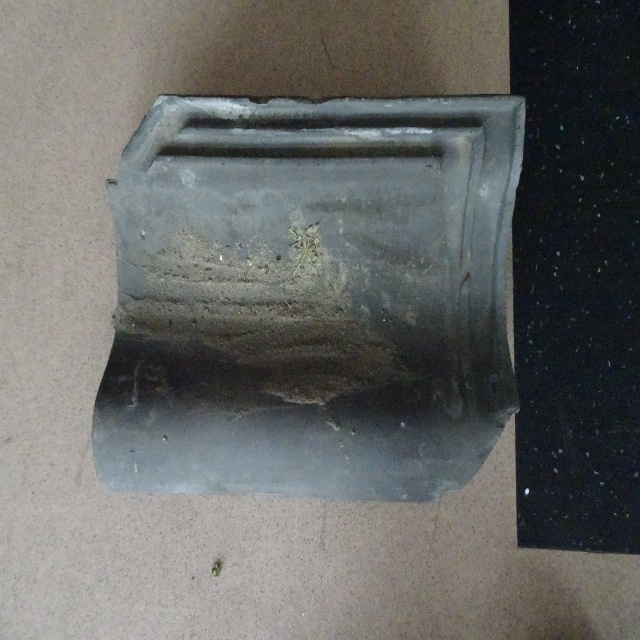
\includegraphics[width=\linewidth]{square_dataset/square0.JPG}
	\caption{An example of a resized image that is stretched.}
	\label{stretched_1}
\end{marginfigure}

\begin{marginfigure} % Use the marginfigure environment for figures to be output to the margin
	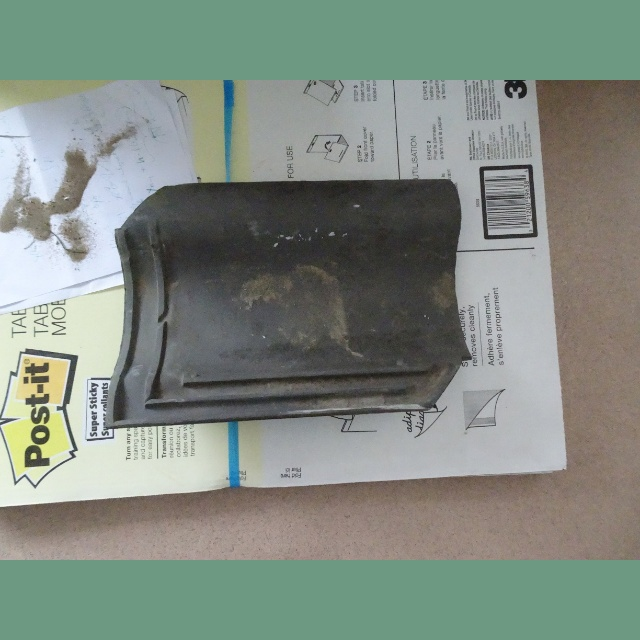
\includegraphics[width=\linewidth]{square_dataset/square1.JPG}
	\caption{Another example of a stretched image.}
	\label{stretched_2}
\end{marginfigure}

\subsubsection{Padding}
To convert non-square images to square ones, we will add a padding to the images depending on the aspect ratio (see images \ref{padding_1} and \ref{padding_2}). The colour of the padding will be random to prevent biases.

\begin{marginfigure} % Use the marginfigure environment for figures to be output to the margin
	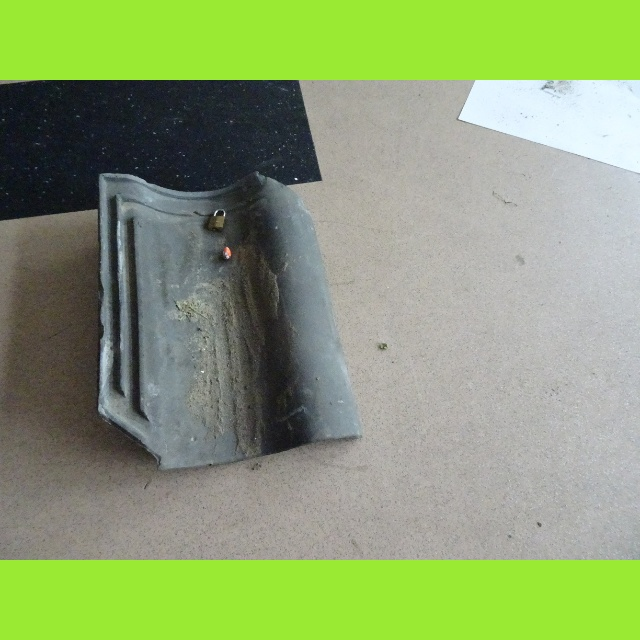
\includegraphics[width=\linewidth]{square_dataset/square2.JPG}
	\caption{Example of a resized image.}
	\label{padding_1}
\end{marginfigure}

% \subsubsection{Padding images}
Instead of stretching the image to the desired aspect ratio, we will add a black background to the non-square images but to make sure adding single colour background does not add bias to images, we will use a random colour for the background. 
In the code, the target resolution is $640*640$ pixels. This resolution is required by most YOLO-models which could be used as the main algorithm classifying the rooftiles. 
To the side are a few examples of images converted to a square aspect ratio.

\begin{marginfigure} % Use the marginfigure environment for figures to be output to the margin
	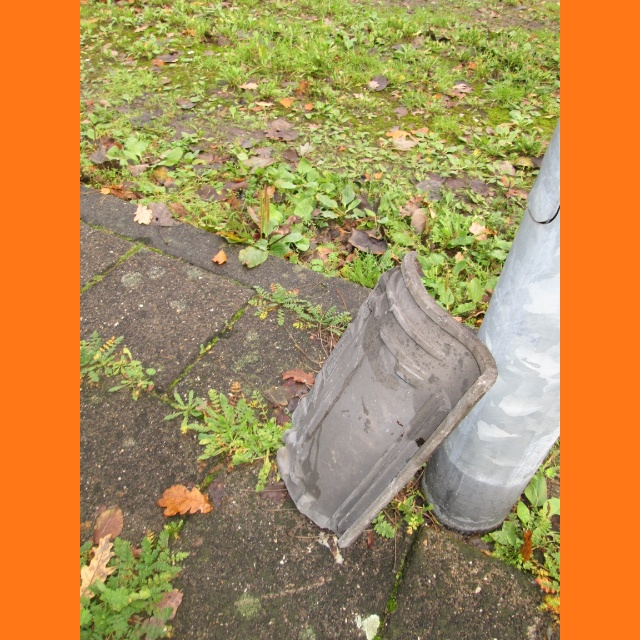
\includegraphics[width=\linewidth]{square_dataset/square3.JPG}
	\caption{Example of a vertical image.}
	\label{padding_2}
\end{marginfigure}

\subsubsection{Padding calculation}
To explain how the resizing is done, 
consider an image with a resolution of $1000*1200$ pixels. 
To make this resolution into the desired $640*640$ image, 
we first have to add $100$ pixels of padding to either horizontal side of the image to make the resolution $1200*1200$. 
After this is done, we resize the image with a factor of $\frac{8}{15}$ to get the desired resolution of $640*640$.
% we have to resize it by a factor of $1/3$ since (it is the minimum of $600/1800 = 1/3$ and $600/1200 = 1/2$). 
% After resizing the original image by a factor of $1/3$, we get to a $600*400$ image. 
% To make this image square, we need to add $120$ pixels of padding to each side of the image to get a $640*640$ resolution.


% \begin{marginfigure} % Use the marginfigure environment for figures to be output to the margin
% 	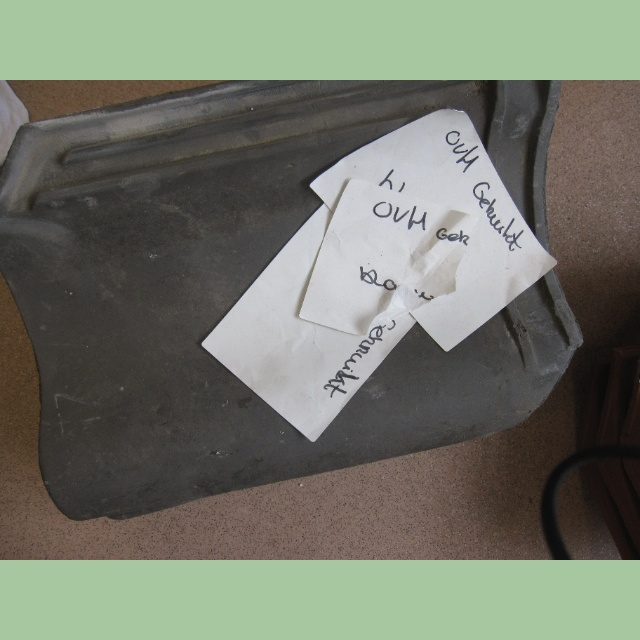
\includegraphics[width=\linewidth]{square_dataset/square5.JPG}
% 	\caption{Square5}
% \end{marginfigure}

\newpage
\subsection{Data augmentation}

\begin{marginfigure}
	% \centering
	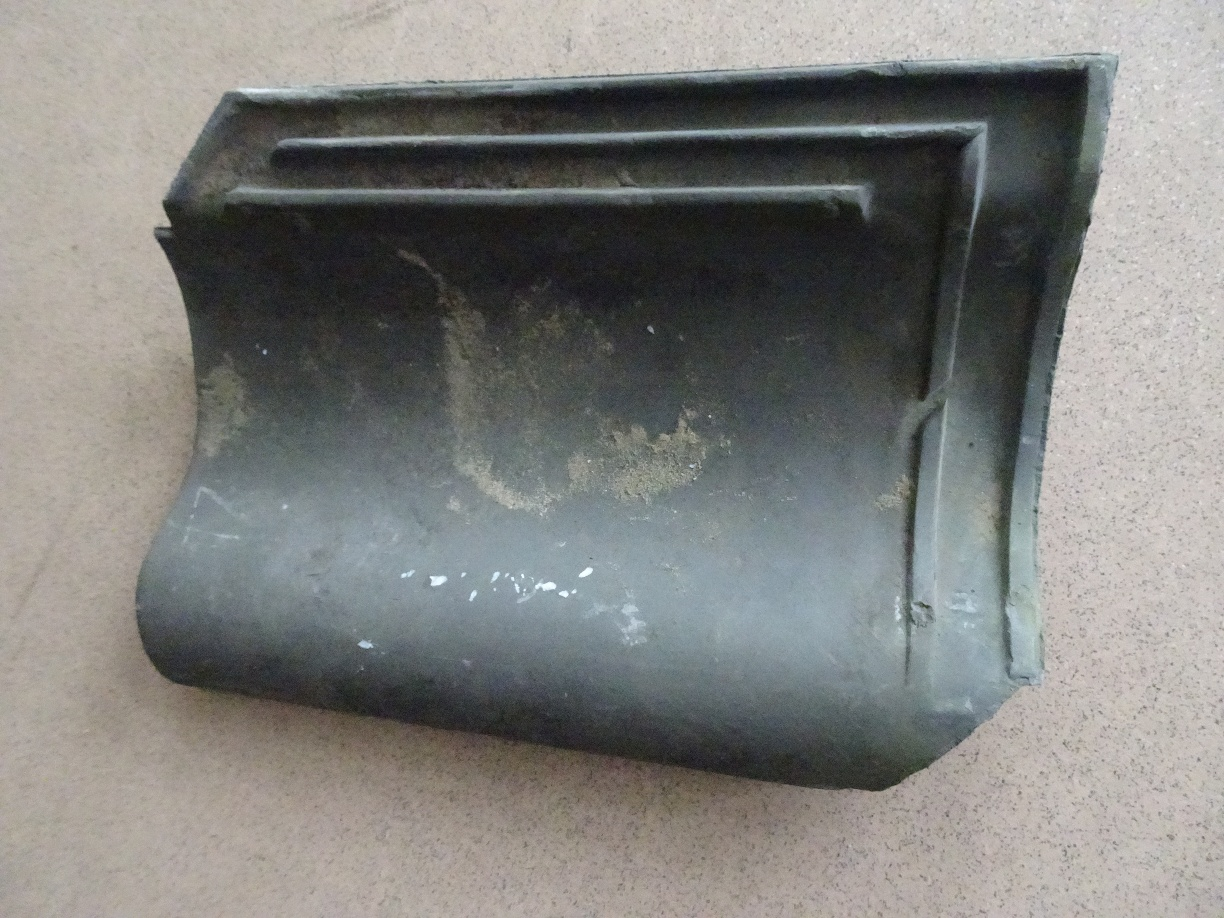
\includegraphics[width=\textwidth]{original.jpg}
	\caption{Original.}
\end{marginfigure}

\begin{marginfigure}
	% \centering
	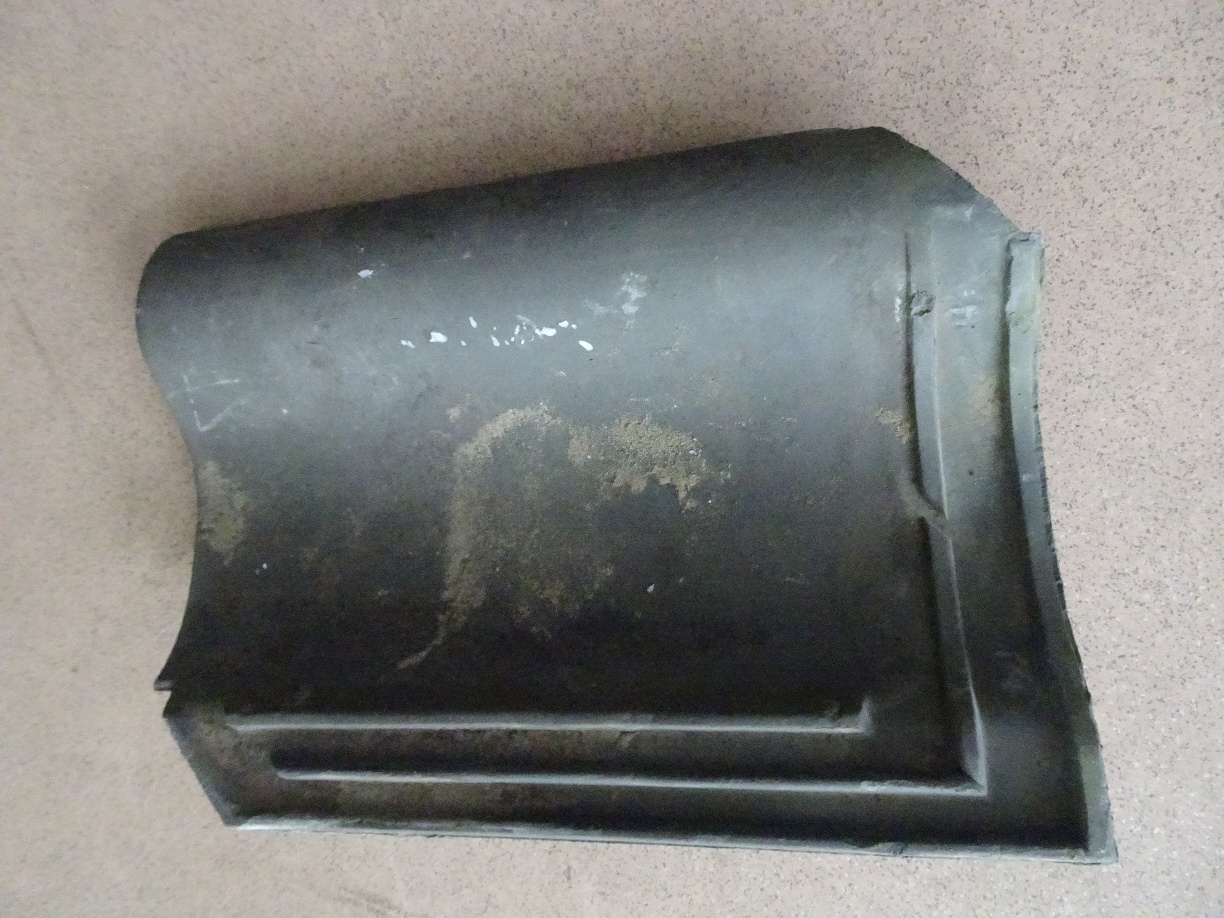
\includegraphics[width=\textwidth]{vertical_flip.jpg}
	\caption{$180^{\circ}$ rotation.}
\end{marginfigure}

\begin{marginfigure}
	% \centering
	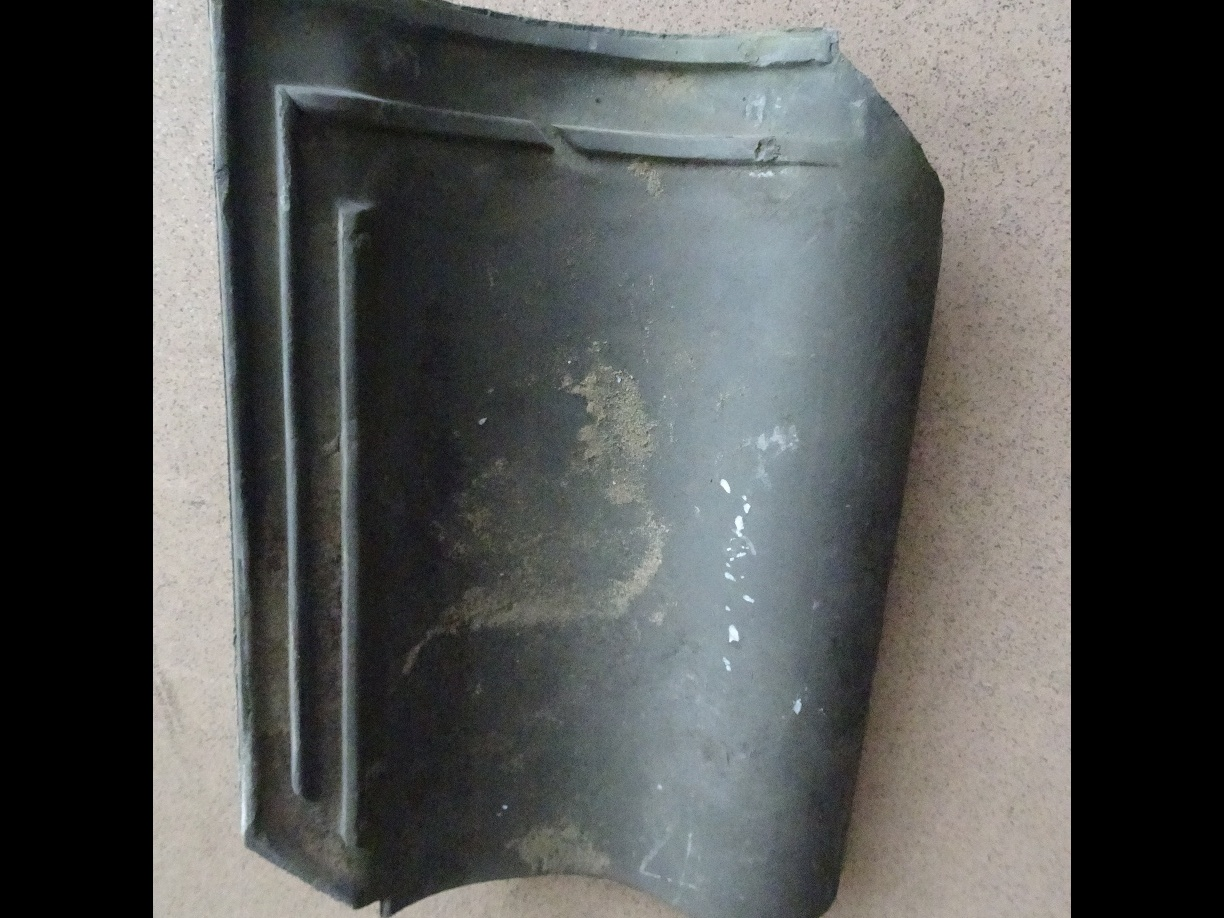
\includegraphics[width=\textwidth]{random_rotation.jpg}
	\caption{$270^{\circ}$ rotation including padding to keep it square.}
\end{marginfigure}

\begin{marginfigure}
	% \centering
	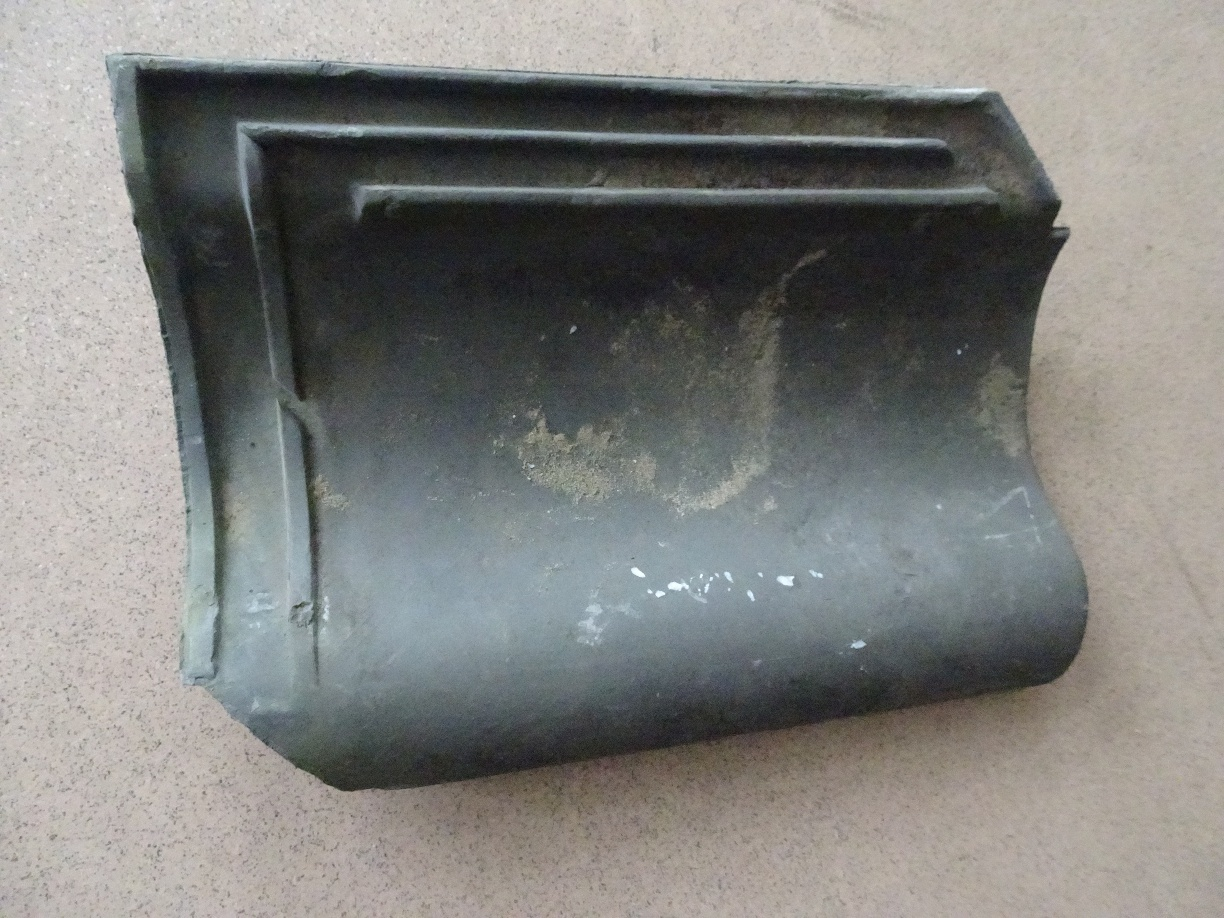
\includegraphics[width=\textwidth]{horizontal_flip.jpg}
	\caption{Horizontal mirroring.}
\end{marginfigure}

\begin{marginfigure}
	% \centering
	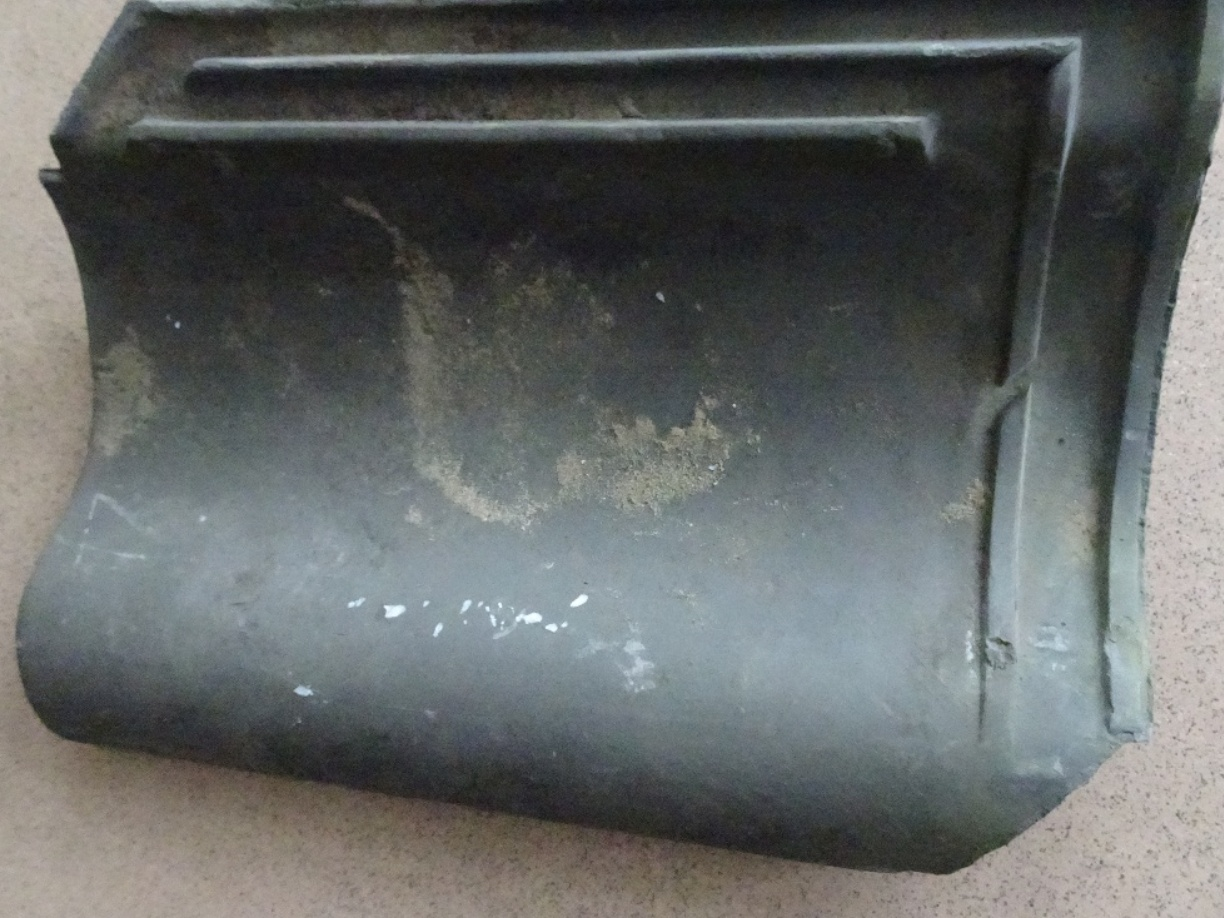
\includegraphics[width=\textwidth]{random_zoom.jpg}
	\caption{Zooming in.}
\end{marginfigure}

% \begin{fullwidth}
A few augmentation techniques are applied to artificially increase the dataset and training data. 
It's important to realize that this is just done for training and not testing, 
since testing requires the images to be as closely to the real world as possible. 
The primary goal of data augmentation is to increase the diversity of the training dataset. 
By doing all techniques below we can create 3 augmented versions of each image within the dataset, provided that the images aren't too similar.
% \end{fullwidth}

\subsubsection{Mirroring}
Mirroring is a common data augmentation technique that is used to either horizontally or vertically mirror an image. 
Even though in the real world the rooftiles don't have a mirrored version of itself, 
it's still a good idea to include this kind of augmented data in the trainingset to improve diversity even more.

\subsubsection{Rotation}
Wihin the realm of rotation, we will use 3 types of a rotated image: $90^{\circ}$, $180^{\circ}$ and $270^{\circ}$. 
All rotations will be done clockwise.

\subsubsection{Zooming}
We will also add zoomed in version of images. Zooming is done until the rooftile barely fits the image. 


%----------------------------------------------------------------------------------------
%	FIGURES EXAMPLE
%----------------------------------------------------------------------------------------

% \section{Figure Examples}

% This statement automatically references the figure below using its label: Figure \ref{fig:example}.

%------------------------------------------------

% \begin{marginfigure} % Use the marginfigure environment for figures to be output to the margin
% 	
\includegraphics[width=\linewidth]{placeholder.jpg}
% 	\caption{Margin figure caption.}
% \end{marginfigure}

% %------------------------------------------------

% \begin{figure}[H] % [H] forces the figure to be output where it is defined in the code (it suppresses floating)
% 	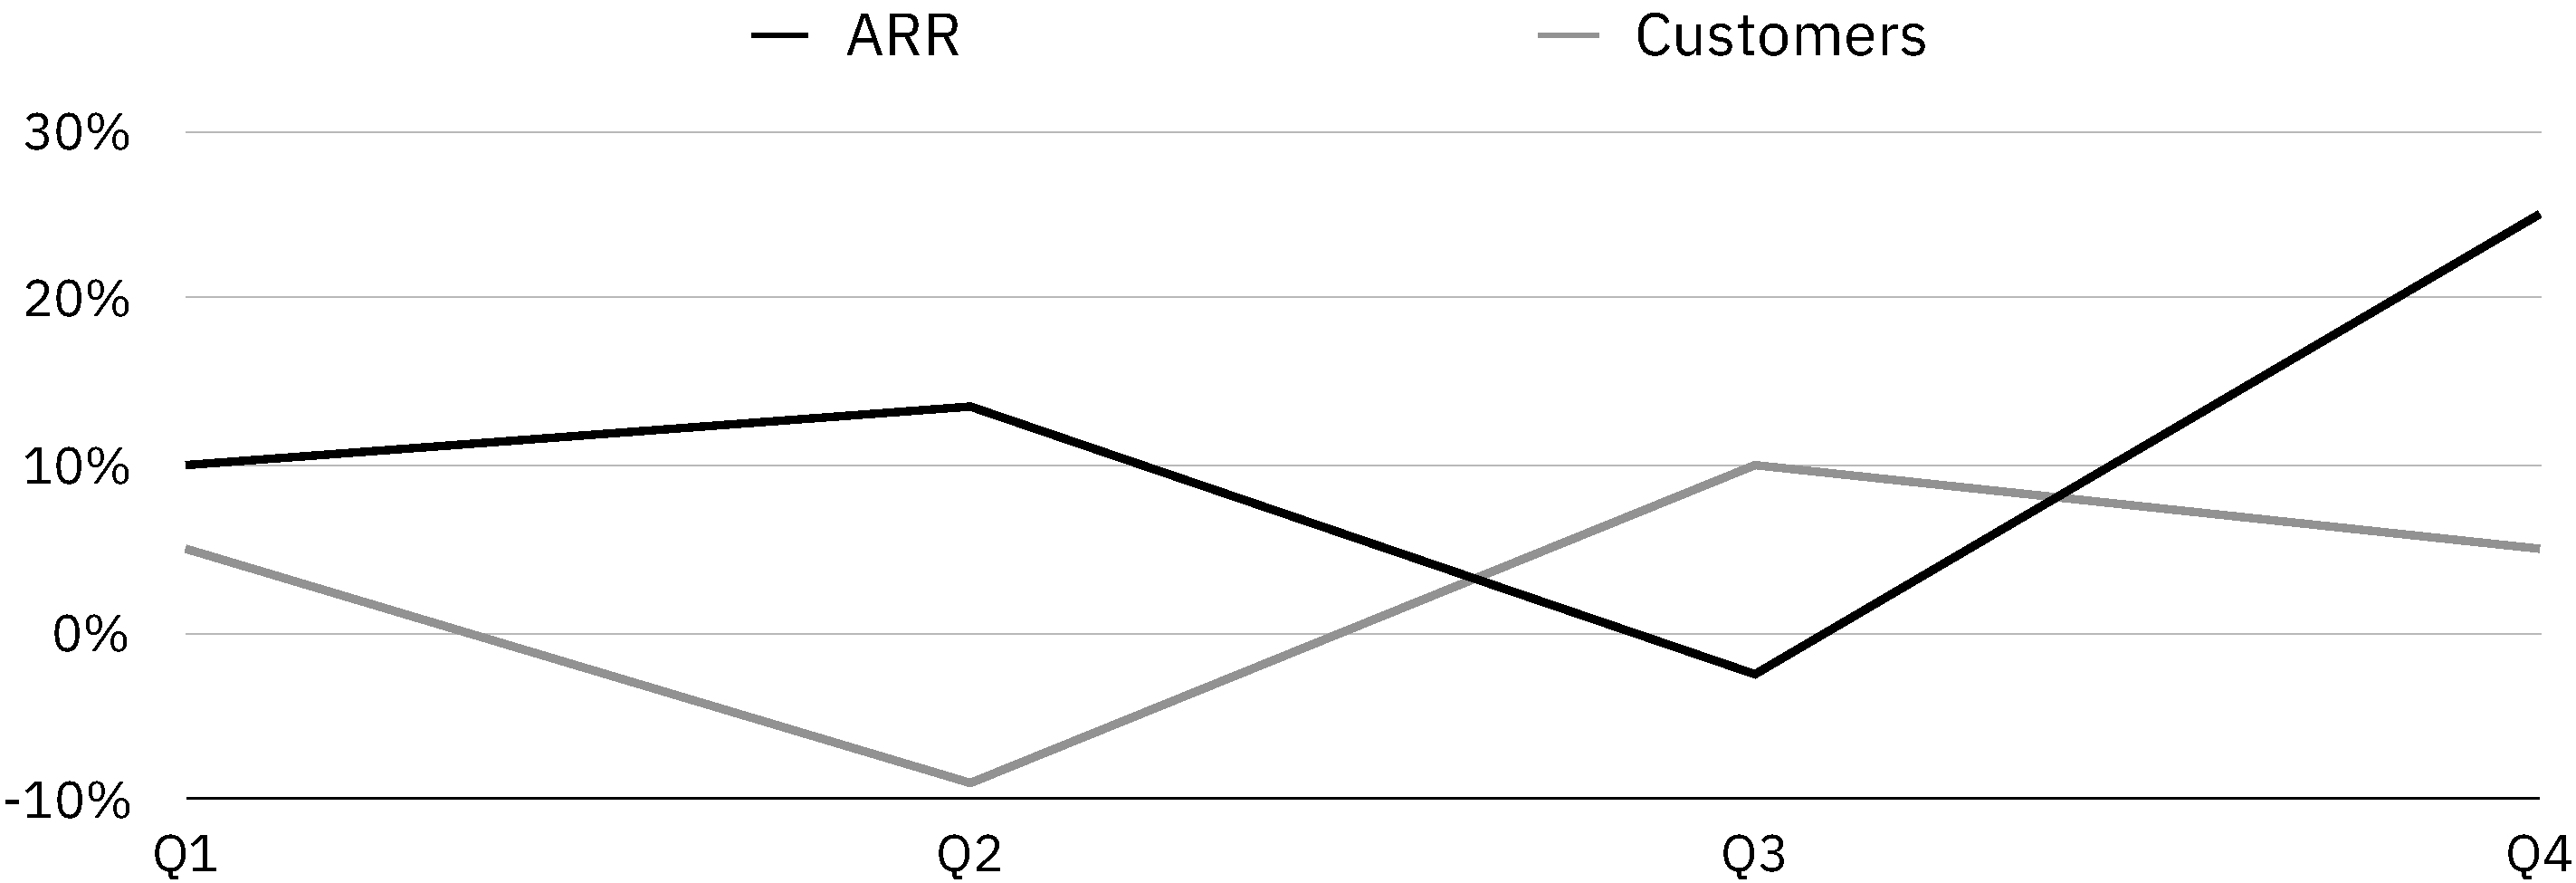
\includegraphics[width=\linewidth]{ARR.pdf}
% 	\caption{Text block figure caption.}
% 	\label{fig:example} % Label for referencing this figure in the text automatically
% \end{figure}

% %------------------------------------------------

% \begin{figure*} % Use the figure* environment for full width figures
% 	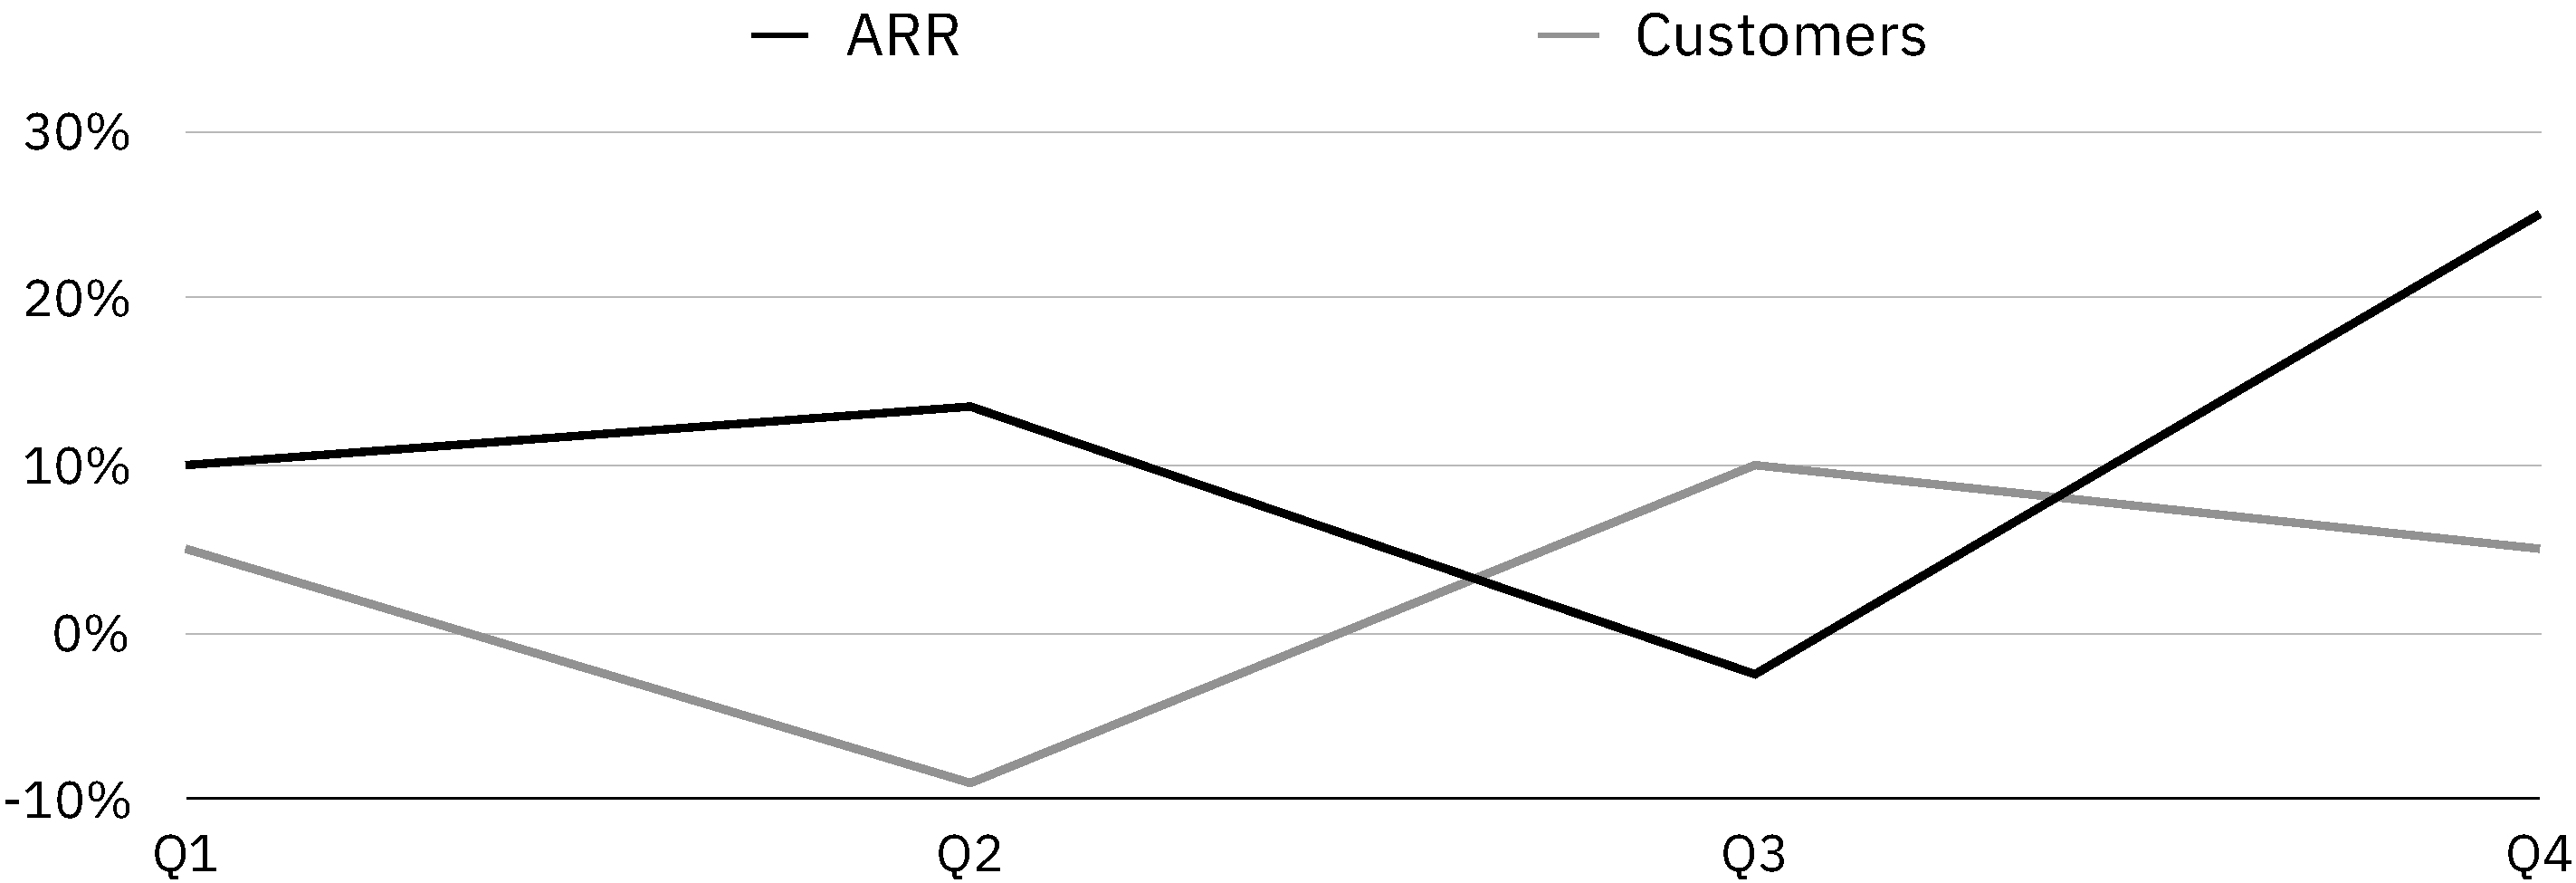
\includegraphics[width=\linewidth]{ARR.pdf}
% 	\caption{Full width figure caption.}
% \end{figure*}

%----------------------------------------------------------------------------------------
